\documentclass[11pt]{article}
\usepackage[margin=1in]{geometry}
\usepackage{amsmath,amssymb}
\usepackage{graphicx}
\usepackage{booktabs}
\usepackage{lmodern}
\usepackage[expansion=false]{microtype}
\usepackage[numbers,sort&compress]{natbib}
\usepackage{xcolor}
\usepackage[colorlinks=true,linkcolor=blue!60!black,citecolor=blue!60!black,urlcolor=blue!60!black]{hyperref}

\title{Scramble Inversion Beyond Groups:\\
Mapping Where Denoising Diffusion Solves Sequential Decision Problems}

\author{Aamer Khani\thanks{Experiments, implementation, and manuscript
preparation were carried out with the assistance of Claude (Anthropic).
Correspondence: \texttt{aamer.khani.1@gmail.com}.}}
\date{August 2026}

\begin{document}
\maketitle

\begin{abstract}
Scramble inversion---train a denoiser to predict the move that undoes the
last step of a random walk from the goal, then solve by reverse-process
rollout---matches or beats deep approximate value iteration (DAVI) on the
Rubik's Cube at a fraction of the compute~\citep{khani2026}. Is this an
accident of the cube's structure, or does ``any RL problem can be a diffusion
problem''? We test the hypothesis with an \emph{assumption ladder}: five
domains, each removing one property the cube quietly provides---group
structure (24-puzzle), a fixed environment and goal (procedural mazes),
invertible actions (Sokoban), discreteness (pendulum swing-up), and
determinism (2048)---each with a matched-architecture, matched-compute value
baseline on one consumer GPU. The map that emerges is sharp. At scale on
reversible discrete spaces the recipe dominates: on the 24-puzzle
($7.7\times10^{24}$ states) the denoiser solves $100\%$ of thousand-move
scrambles ($99.8\%$ with no search at all) while DAVI solves $0.6\%$ at
matched iterations---yet on the exhaustible 8-puzzle both reach $100\%$ and
DAVI is near-optimal, locating the crossover at state-space scale.
Per-instance goal conditioning (mazes) is a tie. Irreversibility flips the
result: reverse (pull-based) walks cannot demonstrate deadlocks, so the
denoiser pushes boxes into corners it can never leave ($66\%$ vs.\ DAVI's
$83\%$). Continuous actions break naive $\epsilon$-\emph{regression}
entirely ($0\%$ swing-up: the bimodal undo-torque posterior collapses to its
useless mean) but not the framing---the same data with a 21-bin categorical
head reaches $100\%$, isolating distributional output, not discreteness, as
the requirement. Stochastic dynamics (2048) defeat the recipe outright: the
denoiser plays at the level of uniform random moves. The hypothesis
therefore survives in a refined form: scramble inversion is the method of
choice for large, deterministic, reversible, goal-reaching problems---and we
give mechanisms, not just scoreboards, for each boundary.
\end{abstract}

\section{Introduction}

A companion study~\citep{khani2026} showed that the Rubik's Cube can be solved by
treating scrambling as the forward process of a discrete diffusion model:
random generator moves are the noise, the scramble depth is the timestep, and
a denoiser trained by cross-entropy to predict the inverse of the last
scramble move solves cubes by reverse-process rollout, matching DAVI's
$100\%$ solve rate at $2.8\times$ less training wall-clock with $5\times$
cheaper iterations. The natural next question---posed by the strong form of
the hypothesis, ``\emph{every} RL problem can be done as diffusion, and may
train faster''---is which properties of the cube that result actually used.

The cube provides five such properties simultaneously: (i) its moves form a
\emph{group} acting freely on states; (ii) there is a \emph{single, fixed
goal} in a \emph{fixed environment}; (iii) every action is
\emph{invertible}; (iv) states and actions are \emph{discrete}; (v) dynamics
are \emph{deterministic}. Rather than accumulate more successes on
cube-like puzzles, we designed one domain per removed assumption
(Table~\ref{tab:ladder}) and ran the identical recipe against a
matched-architecture value-learning baseline in each, all on one RTX~5080
laptop GPU, with the same verification discipline as the companion paper
(exact oracles where the space permits; every claimed solution replayed in
the environment).

\begin{table}[t]
\centering
\small
\begin{tabular}{llll}
\toprule
Domain & Removes & Winner & Mechanism \\
\midrule
8-puzzle ($1.8\times10^5$) & --- (control) & tie ($100\%$/$100\%$) & value memorizes small spaces \\
24-puzzle ($7.7\times10^{24}$) & group structure & \textbf{denoiser} ($100\%$ vs $0.6\%$) & bootstrap can't reach depth \\
Mazes (procedural) & fixed goal/env & tie ($76\%$/$77\%$) & conditioning taxes both \\
Sokoban & invertibility & \textbf{value} ($83\%$ vs $66\%$) & reverse data is deadlock-blind \\
Pendulum & discreteness & tie$^{*}$ ($100\%$/$100\%$) & $^{*}$only with distributional head \\
2048 & determinism & \textbf{neither} (denoiser $=$ random) & reverse process models the wrong game \\
\bottomrule
\end{tabular}
\caption{The assumption ladder and outcomes. ``Winner'' refers to greedy
(search-free) solving under matched training; see the domain sections for
full protocols.}
\label{tab:ladder}
\end{table}

\begin{figure}[t]
\centering
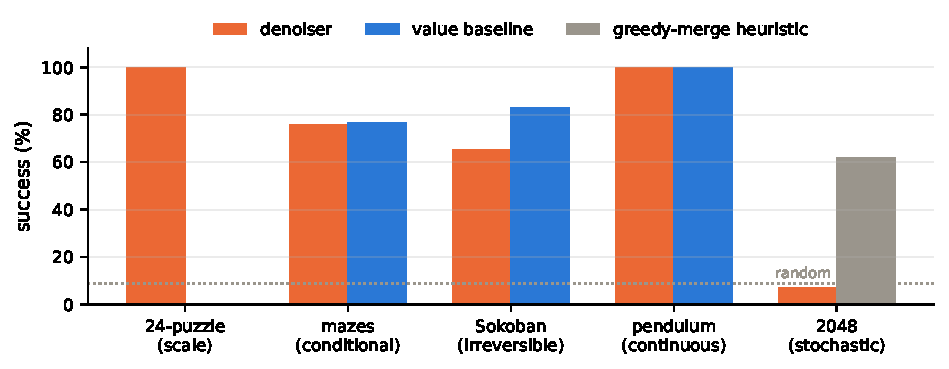
\includegraphics[width=0.92\linewidth]{fig2_summary.pdf}
\caption{Headline success rates across the ladder (orange: denoiser; blue:
matched value baseline; gray: 2048 heuristic reference, dotted line: random
play). Success metric per domain: 24-puzzle and Sokoban (depth 60), solve
rate; mazes, fresh-instance solve rate; pendulum, swing-up-and-hold;
2048, reaching the 256 tile.}
\label{fig:summary}
\end{figure}

Our contribution is not a new algorithm but a \emph{boundary map with
mechanisms}: each domain isolates one assumption, each outcome comes with an
ablation or diagnostic that explains it, and all code, logs, and per-domain
result files are released.

\section{The recipe and its five pillars}
\label{sec:recipe}

Given an environment with goal set $G$, the scramble-inversion recipe is:
(1) sample a noising walk $s_0 \in G,\; s_k = T(s_{k-1}, a_k)$ where $T$ is a
\emph{reverse} transition kernel and $a_k$ random noise ops, with depth
$t \sim \mathrm{Unif}\{1..K\}$ (linear schedule); (2) train
$p_\theta(\,\cdot\mid s_t)$ by cross-entropy (or regression) to predict the
forward action that undoes $a_t$; (3) act by greedy rollout of $p_\theta$,
optionally with beam search. The five pillars are where each step can break:
step (1) needs a way to run dynamics \emph{backward from the goal}
(invertibility or an auxiliary reverse kernel), and needs the induced state
distribution to resemble states met at solve time (determinism); step (2)
needs the undo-posterior's summary (argmax or mean) to be a good action
(discreteness/distributional output); step (3) needs the goal to be reachable
by local descent (scale is the denoiser's friend here, and the value
baseline's enemy). The domains below stress each in turn. Baselines are DAVI
with the identical backbone (residual MLP, LayerNorm), batch (8--10k), Adam,
and schedule, differing only in head and objective, exactly as in the
companion paper.

\section{Results along the ladder}

\subsection{Scale without group structure: sliding-tile puzzles}

The 15/24-puzzle family drops the group property (legal moves depend on the
blank's position) while keeping everything else. On the \textbf{8-puzzle},
whose 181{,}440 states we sweep exhaustively against an exact BFS oracle,
\emph{both} methods solve $100\%$ of all states greedily; DAVI is nearly
optimal (avg.\ 21.99 moves vs.\ optimum 21.97; $99.5\%$ of its argmax moves
reduce true distance) while the denoiser gives up $\sim$1 move ($88.7\%$).
Small spaces are value iteration's best case: the scalar function can be
learned everywhere. On the \textbf{24-puzzle} ($7.7\times10^{24}$ states,
scrambles of 1000 moves), the picture inverts completely
(Figure~\ref{fig:slide24}): the denoiser reaches $100\%$ greedy solve rate
on every probe depth by 60k iterations ($\sim$1.9\,h) and solves
$500/500$ evaluation scrambles ($99.8\%$ with no search; avg.\ 139.6 moves);
DAVI at matched iterations solves $0.6\%$, its bootstrapped values never
propagating to the depths where scrambles live. Scale, not group structure,
is what the cube result needed.

\begin{figure}[t]
\centering
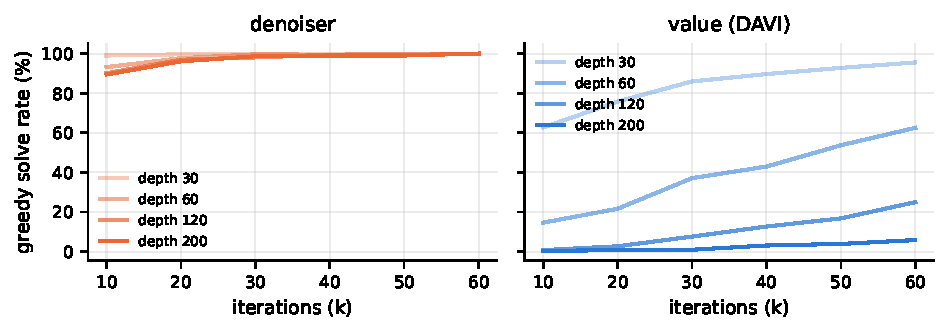
\includegraphics[width=0.9\linewidth]{fig2_slide24.pdf}
\caption{24-puzzle greedy solve rate during training by scramble depth
(left: denoiser; right: DAVI, same axes). The denoiser saturates all depths
by 60k iterations; DAVI's coverage grows outward from the goal and reaches
$6\%$ at depth 200 by the matched budget.}
\label{fig:slide24}
\end{figure}

\subsection{Conditioning: procedural mazes}

With a fresh random obstacle grid and goal cell per instance, the denoiser
becomes conditional, $p_\theta(a \mid s, \mathrm{maze})$---the analogue of
conditional diffusion. On 20k held-out instances with starts sampled
uniformly over reachable cells (exact per-instance BFS oracles), the methods
tie: $76.0\%$ (denoiser) vs.\ $76.6\%$ (DAVI), with DAVI's paths closer to
optimal ($1.05\times$ vs.\ $1.21\times$ the exact distance) and the denoiser
$4\times$ faster to evaluate. Per-instance conditioning taxes both methods
equally; neither the diffusion framing nor value bootstrapping has a
structural advantage here.

\subsection{Irreversibility: Sokoban}

Sokoban's pushes cannot be undone, so the noising walk uses \emph{pulls}
(reverse dynamics available only at training time); every generated instance
is solvable by construction, which we verify by replaying each pull sequence
backward as pushes. The value baseline wins at every depth
(Figure~\ref{fig:sokoban}): $83.1\%$ vs.\ $66.5\%$ at pull-depth 60. The
mechanism is visible in the construction itself: \emph{reverse walks can
never enter a deadlock} (a pulled box is never against a wall it cannot
leave), so the denoiser's data contains no signal about which pushes are
fatal, and its failures are dominated by boxes pushed into corners. DAVI's
bootstrap runs through the \emph{forward} dynamics, so dead states keep high
cost-to-go and are avoided. When actions are irreversible, learning from
reverse experience alone is structurally blind to exactly the mistakes that
matter.

\begin{figure}[t]
\centering
\begin{minipage}{0.48\linewidth}
\centering
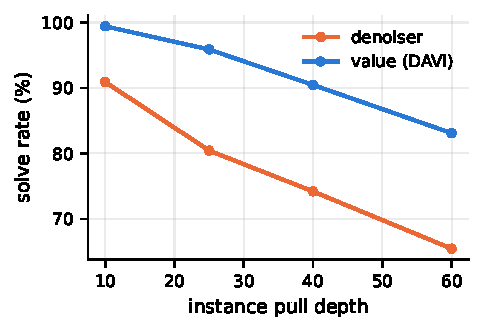
\includegraphics[width=\linewidth]{fig2_sokoban.pdf}
\end{minipage}\hfill
\begin{minipage}{0.48\linewidth}
\centering
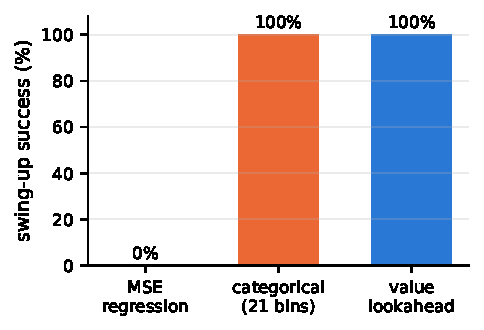
\includegraphics[width=\linewidth]{fig2_pendulum.pdf}
\end{minipage}
\caption{\textbf{Left (Sokoban):} solve rate vs.\ instance difficulty; the
gap is deadlock-blindness of reverse-only training. \textbf{Right
(pendulum):} the continuous ablation --- $\epsilon$-regression collapses to
the bimodal posterior's mean ($0\%$); the same data and backbone with a
21-bin categorical head reaches $100\%$; value lookahead also $100\%$.}
\label{fig:sokoban}
\end{figure}

\subsection{Continuity: pendulum swing-up}

For the underactuated pendulum ($u_{\max}=2 < mgl = 10$), the noising
process integrates the dynamics backward in time from upright under random
torques---the reverse step is the exact inverse of the semi-implicit Euler
forward step (error $<10^{-6}$), so every noising trajectory is a genuine
forward trajectory reversed. Naive $\epsilon$-\emph{regression} fails
totally ($0\%$ swing-up from hanging, 2048 episodes): near the bottom, the
posterior over undoing torques is bimodal (reverse walks spin both ways) and
the MSE-optimal prediction is its mean---zero torque, no energy pumping.
Replacing the scalar head with a 21-bin categorical head---same data, same
backbone, cross-entropy---restores $100\%$ ($75.6$ steps mean); the value
baseline with 1-step lookahead over a torque grid also reaches $100\%$
($63.9$ steps). Continuity per se is not the boundary; \emph{keeping the
distribution} is. This is precisely why diffusion samplers iterate and
sample rather than regress, reproduced here as a two-line ablation.

\subsection{Stochasticity: 2048}

2048 interleaves chosen slides with random tile spawns, and its goal is a
set of states. Our best-faith adaptation trains the denoiser on
deterministic reverse play (tile un-merges and un-spawns from a constructed
256-tile board) and evaluates in the real stochastic game. The result is an
unambiguous failure: the denoiser's play is statistically indistinguishable
from uniform random legal moves (mean max tile 105 vs.\ 109; reaching 256 in
$7.1\%$ vs.\ $9.0\%$ of games), while a one-line greedy-merge heuristic more
than doubles both (238; $61.8\%$). With stochastic dynamics the reverse
process describes a game that is never actually played: the marginal it
induces, and the undo-labels it provides, do not correspond to any policy's
state distribution under real spawns. Determinism is not a convenience of
the recipe; it is a requirement.

\section{Discussion}

\textbf{The refined hypothesis.} ``Every RL problem can be diffusion'' does
not survive; something more useful does. Scramble inversion is the method of
choice when (a) the state space is too large for value bootstrapping to
cover, (b) a faithful reverse kernel exists (invertible actions, or reverse
dynamics whose support matches forward play), (c) dynamics are
deterministic, and (d) the action posterior is represented distributionally.
Condition (a) is not incidental---it is where the method's advantage
\emph{comes from}: the denoiser learns a local descent direction that
transfers across the space, while the value baseline must propagate a global
scalar outward from the goal. Conversely (b) and (c) are hard boundaries
with identified mechanisms (deadlock-blindness; wrong-game marginals), not
tuning problems.

\textbf{Hybrids.} The failures suggest their own fixes, which we leave to
future work: mixing a fraction of \emph{forward} experience into training
(to expose deadlocks), denoiser-proposes/value-scores combinations
(Sokoban, and solution-length polishing generally), and stochastic-aware
reverse processes that marginalize over exogenous noise (2048).

\textbf{Limitations.} Single seed per configuration; one hardware platform;
modest network sizes (1.7M--16M parameters); heuristic rather than learned
baselines for 2048; Sokoban instances from one generator family (8$\times$8,
3 boxes); and our value baselines are greedy/1-step solvers---stronger
search at evaluation time would raise both methods.

\section{Reproducibility}

All five environments are pure-PyTorch and vectorized (10k--200k instances
per batch on one laptop GPU); every domain ships its trainer, evaluator, and
a validation gate that reproduces a known exact quantity (8-puzzle:
181{,}440 states, diameter 31; mazes: BFS field equals Manhattan distance on
empty grids; Sokoban: pull-walks replay to solved under pushes; pendulum:
reverse step inverts forward step to $10^{-6}$; 2048: tile-mass
conservation). Per-domain results are machine-readable JSON in
\texttt{paper2\_data/}. Code:
\url{https://github.com/aamirkhani/rubiks-diffusion}. Total compute for
this study: $\sim$9 GPU-hours.

\begin{thebibliography}{9}

\bibitem[Agostinelli et~al.(2019)]{agostinelli2019}
F.~Agostinelli, S.~McAleer, A.~Shmakov, and P.~Baldi.
\newblock Solving the {R}ubik's cube with deep reinforcement learning and search.
\newblock \emph{Nature Machine Intelligence}, 1(8):356--363, 2019.

\bibitem[Austin et~al.(2021)]{austin2021}
J.~Austin, D.~D. Johnson, J.~Ho, D.~Tarlow, and R.~van~den Berg.
\newblock Structured denoising diffusion models in discrete state-spaces.
\newblock In \emph{NeurIPS}, 2021.

\bibitem[Chi et~al.(2023)]{chi2023}
C.~Chi, S.~Feng, Y.~Du, Z.~Xu, E.~Cousineau, B.~Burchfiel, and S.~Song.
\newblock Diffusion policy: Visuomotor policy learning via action diffusion.
\newblock In \emph{Robotics: Science and Systems}, 2023.

\bibitem[Florensa et~al.(2017)]{florensa2017}
C.~Florensa, D.~Held, M.~Wulfmeier, M.~Zhang, and P.~Abbeel.
\newblock Reverse curriculum generation for reinforcement learning.
\newblock In \emph{CoRL}, 2017.

\bibitem[Ho et~al.(2020)]{ho2020}
J.~Ho, A.~Jain, and P.~Abbeel.
\newblock Denoising diffusion probabilistic models.
\newblock In \emph{NeurIPS}, 2020.

\bibitem[Khani(2026)]{khani2026}
A.~Khani.
\newblock Scramble inversion as discrete denoising diffusion: A
matched-compute study on the {R}ubik's cube group.
\newblock Preprint, 2026.

\bibitem[Sohl-Dickstein et~al.(2015)]{sohldickstein2015}
J.~Sohl-Dickstein, E.~Weiss, N.~Maheswaranathan, and S.~Ganguli.
\newblock Deep unsupervised learning using nonequilibrium thermodynamics.
\newblock In \emph{ICML}, 2015.

\bibitem[Takano(2023)]{takano2023}
K.~Takano.
\newblock Self-supervision is all you need for solving {R}ubik's cube.
\newblock \emph{Transactions on Machine Learning Research}, 2023.

\end{thebibliography}

\end{document}
